\newpage
\subsection{Учет готовой продукции}
\label{bp:readygoods}


Вся готовая продукция поступает на линию упаковки. Водитель погрузчика забирает паллеты с упакованной готовой продукцией на склад ГП. 

На складе ГП есть разметка для ячеечного хранения продукции (рис. \ref{pic:f5}).

Водитель погрузчика расставляет продукцию на складе в свободные ячейки и указывает в ведомости параметры продукции и ячейку, куда поставил ГП (рис. \ref{pic:f7}). В конце смены ведомость передается кладовщику. Кладовщик вносит данные в таблицу MS EXCEL (рис. \ref{pic:f10}).

В конце смены мастер смены заполняет свою ведомость по данным работы производственной  линий (рис. \ref{pic:f6}). По этой ведомости мастер сверяется с данными подаваемыми кладовщиком и подтверждают факт подписями. 


\begin{figure}
\begin{center}
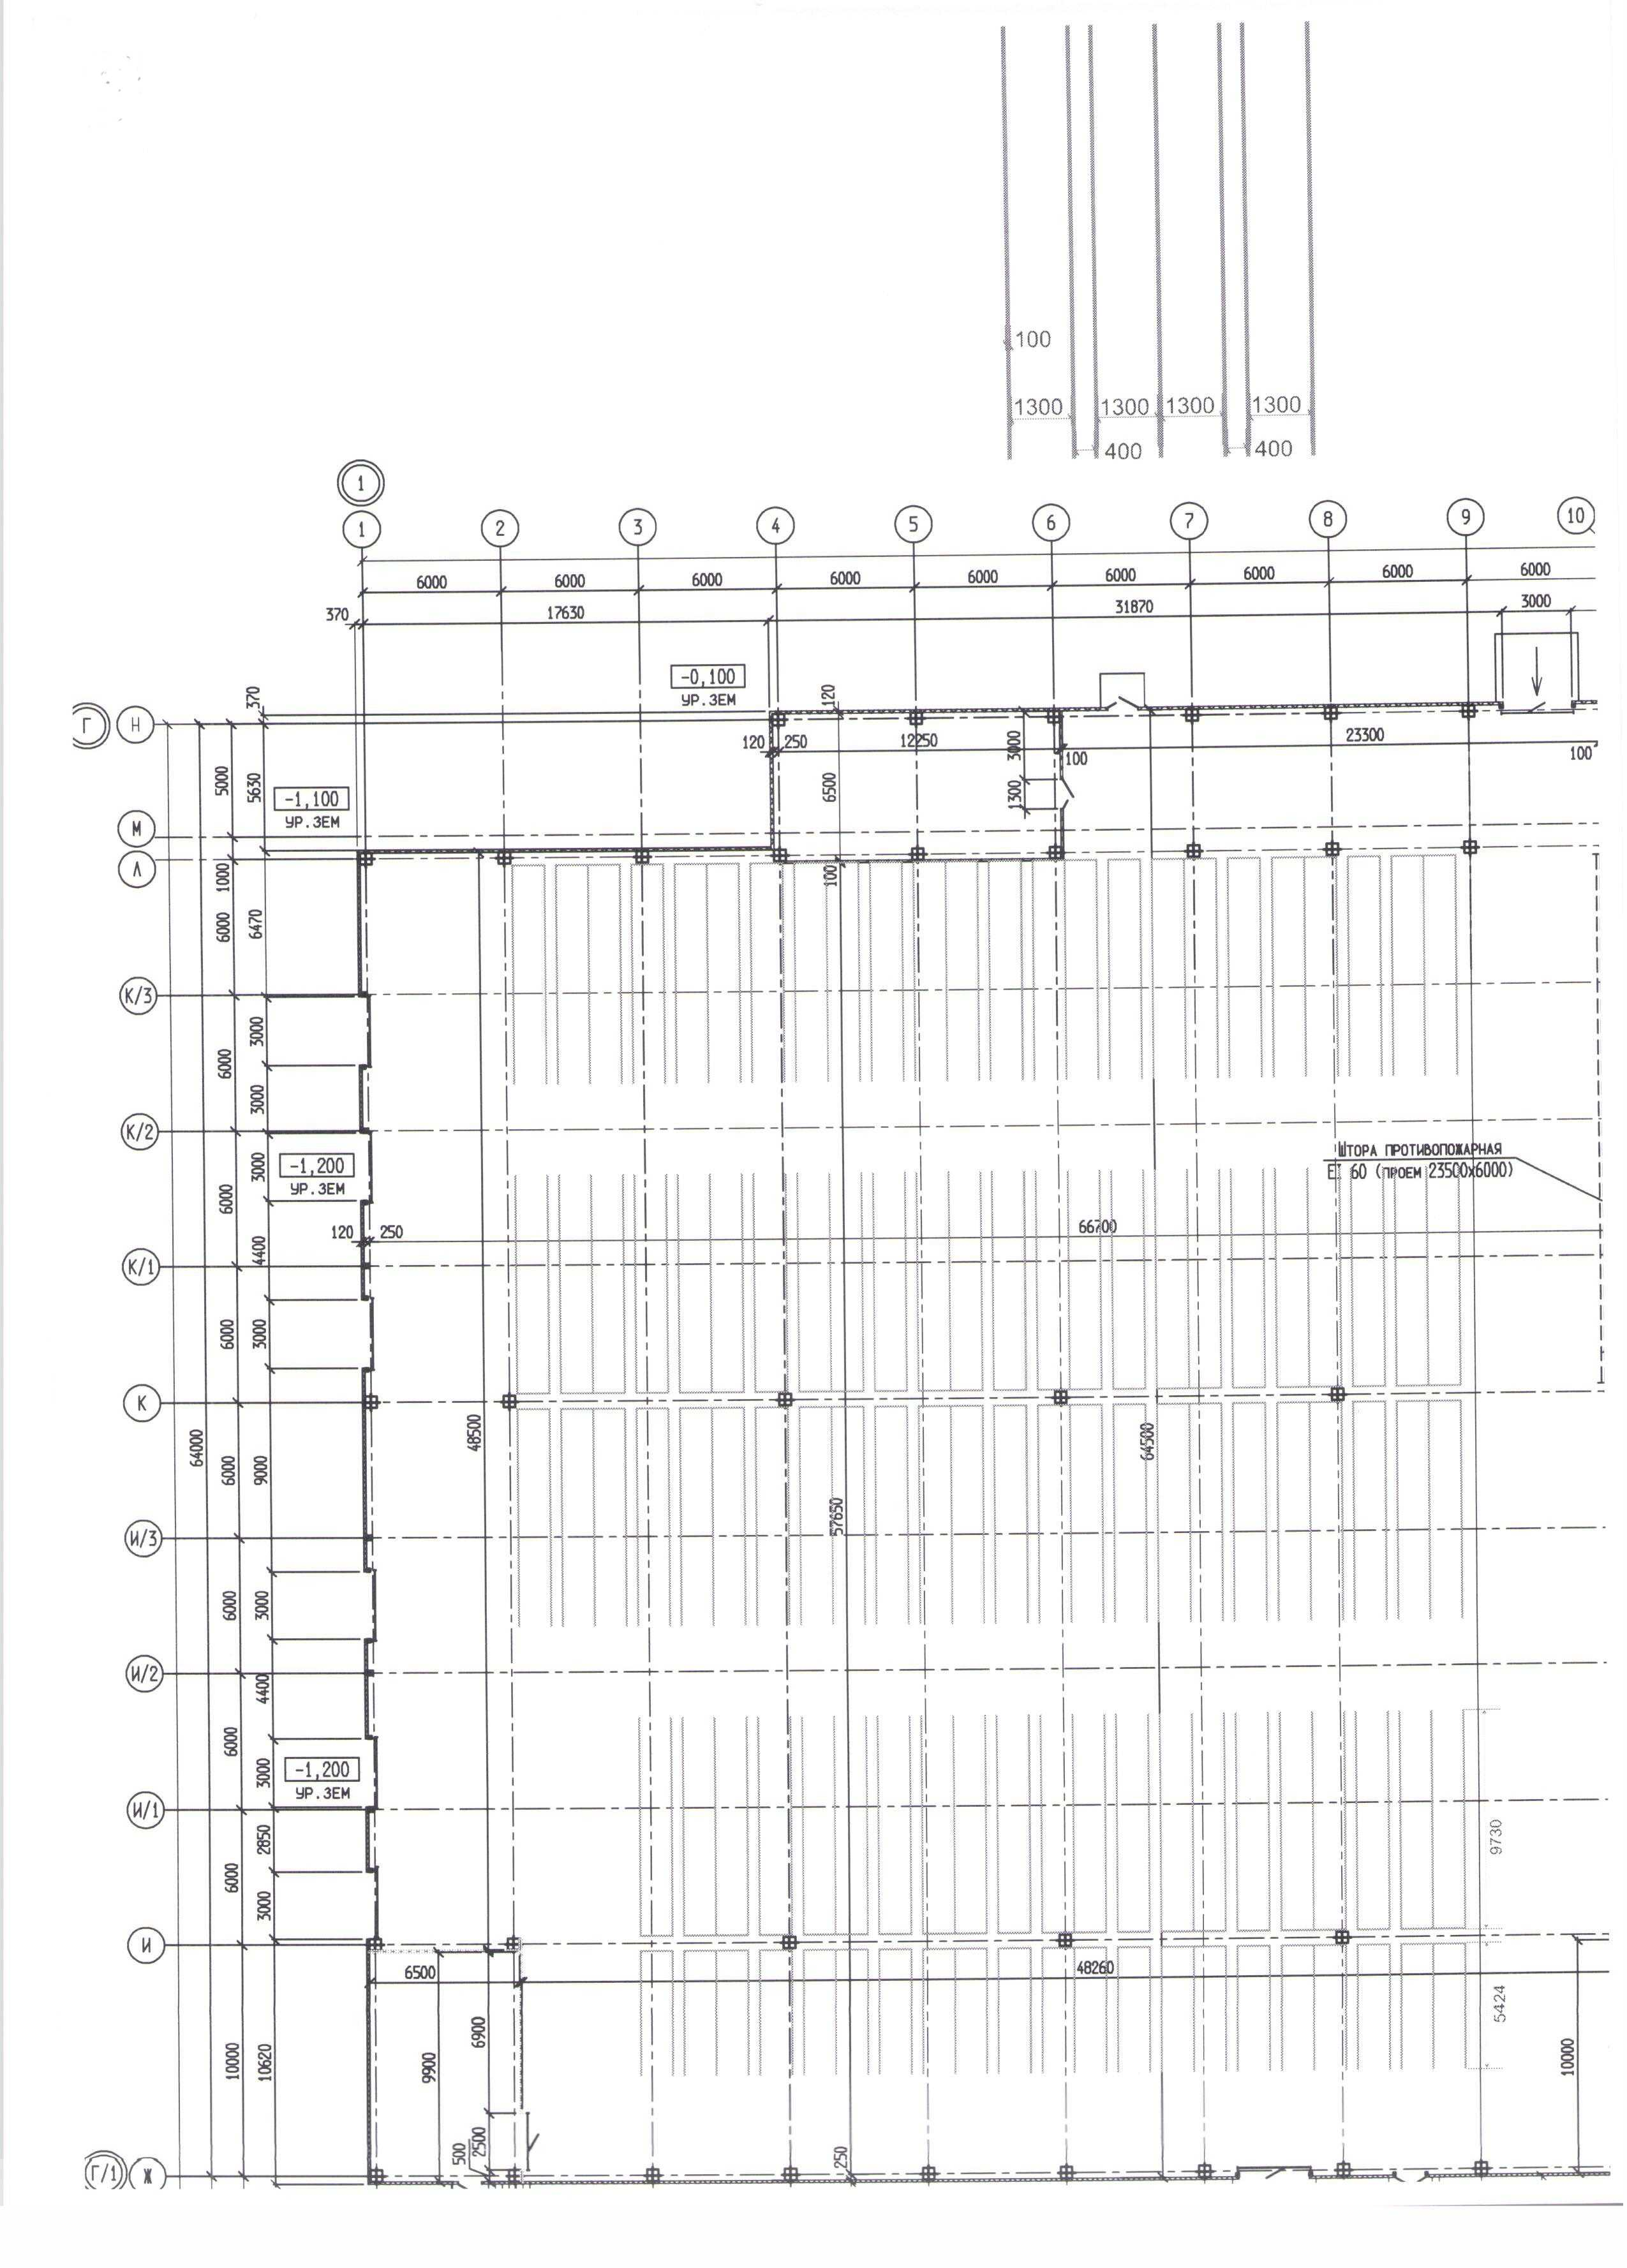
\includegraphics[height=0.94\textheight, width=\textwidth, keepaspectratio]{Pics/f5.jpg}
\end{center}
\caption{Склад ГП. Разметка предусматривающая ячеистое хранение продукции}
\label{pic:f5}
\end{figure}


\begin{figure}
\begin{center}
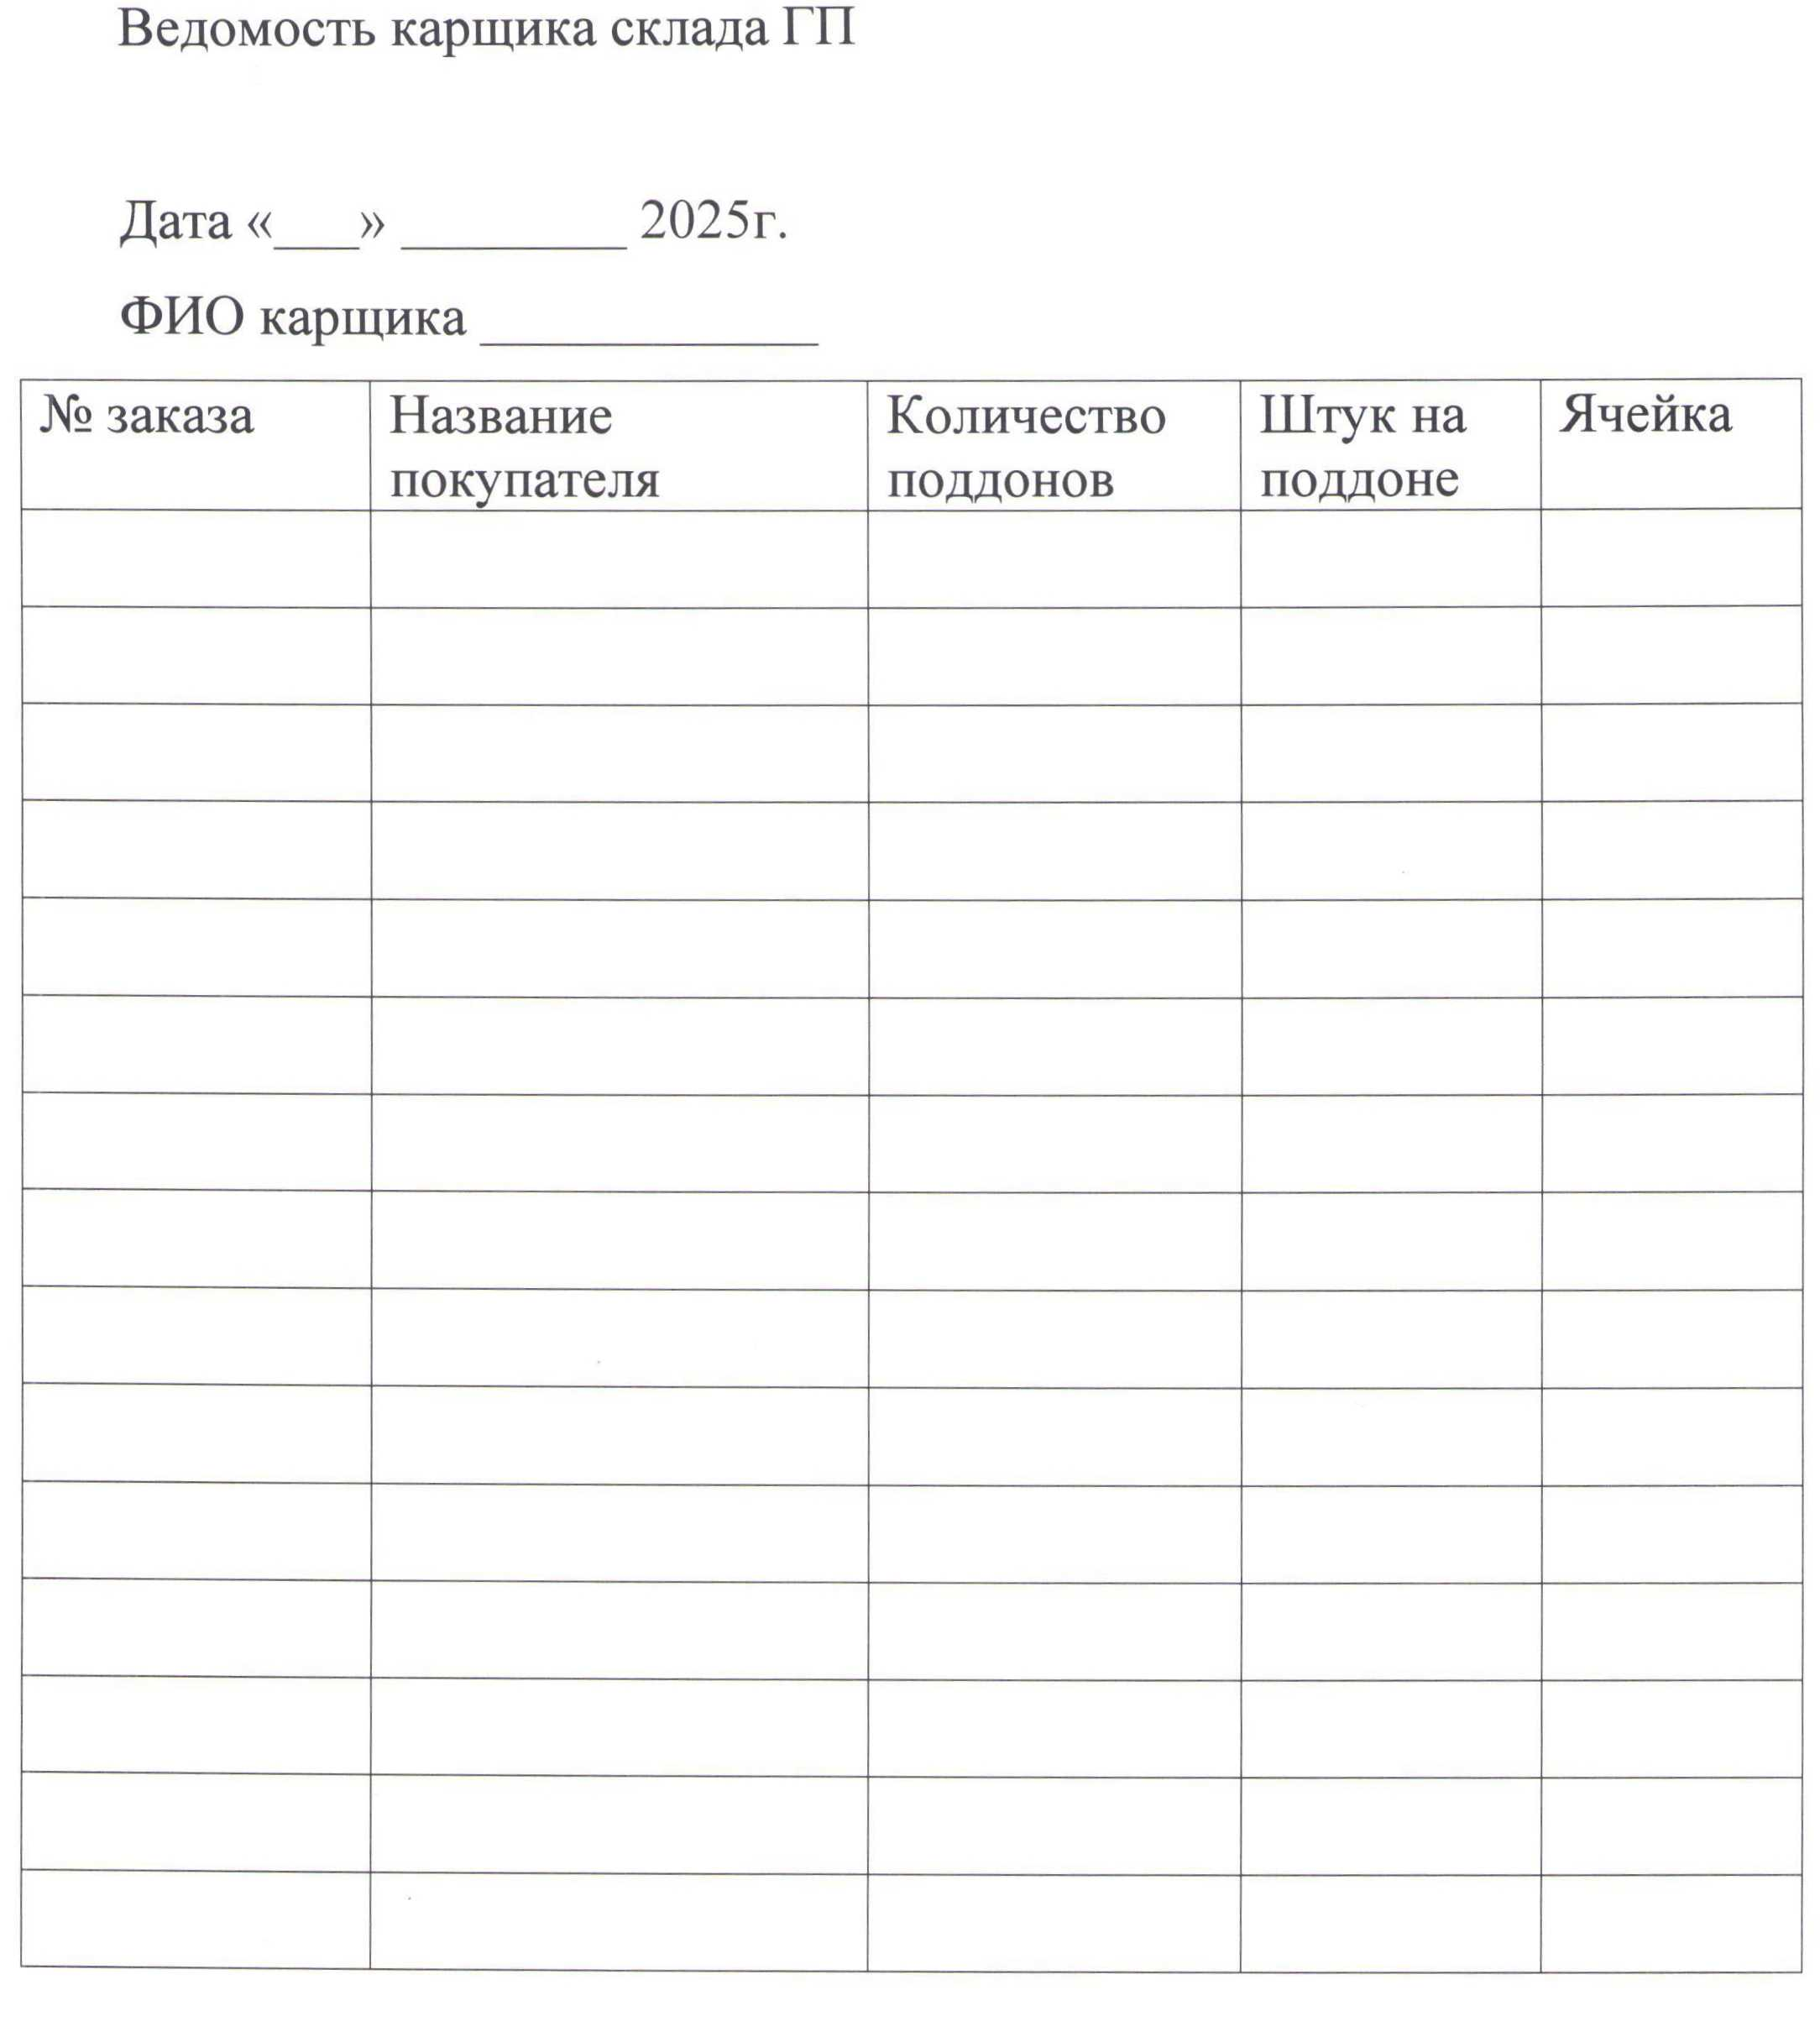
\includegraphics[height=0.94\textheight, width=\textwidth, keepaspectratio]{Pics/f7.jpg}
\end{center}
\caption{Ведомость карщика склада ГП}
\label{pic:f7}
\end{figure}

